\clearpage

\section{Eukliden suorakulmio}

Hirviö Euklides haluaa jakaa suorakulmion muotoisen kivenlohkareen kahteen täydellisesti saman kokoiseen palaan. Palat jakavan leikkaussuoran täytyy kulkea ulkopuolisen pisteen kautta. Euklidella on käytössä ainoastaan täysin suora keppi ja valkoinen liitu. Kuinka Euklides onnistuu?

\begin{figure}[h]
    \centering
    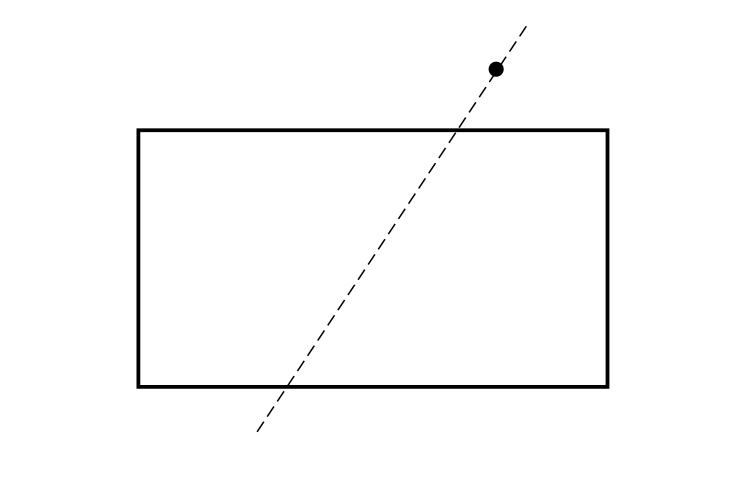
\includegraphics[width=0.6\linewidth]{kuvat/suorakulmio_kahteen_osaan.png}  
\end{figure}